\tikzstyle{entree}=[very thick,black,samples=201]
\tikzstyle{stable}=[very thick,blue,samples=201]
\tikzstyle{instable}=[very thick,red,samples=201]
\tikzsetnextfilename{entree_echelon-chap0_ext}
\begin{tikzpicture}
    \begin{axis}
    [   ticks=none,
        axis line style = thick,
        height=5cm,
        width=5cm,
        axis x line=center,
        axis y line=center,
        xmin=-2,
        xmax=10,
        ymin=-0.5,
        ymax=2.0,
        xlabel={$t$},
        ylabel={$e(t)$},
        xlabel style={below right},
        ylabel style={above left},
    ]
    \addplot[entree,domain=-2:0]  {0};
    \addplot[entree,domain=0:10]  {1};
    \end{axis}
\end{tikzpicture}
\tikzsetnextfilename{stable_echelon-chap0_ext}
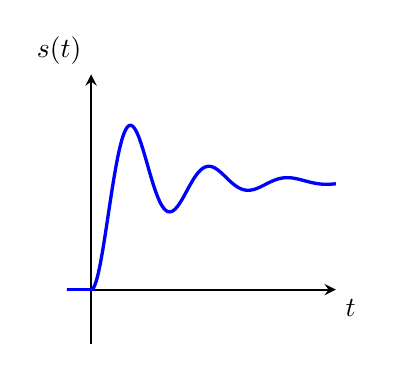
\begin{tikzpicture}
    \begin{axis}
    [   ticks=none,
        axis line style = thick,
        height=5cm,
        width=5cm,
        axis x line=center,
        axis y line=center,
        xmin=-2,
        xmax=20,
        ymin=-0.5,
        ymax=2.0,
        xlabel={$t$},
        ylabel={$s(t)$},
        xlabel style={below right},
        ylabel style={above left},
    ]
    \addplot[stable,domain=-2:0]  {0};
    \def\a{0.3}
    \def\w{0.953939201417}
    \def\p{1.26610367278}
    \def\a{0.2}
    \def\w{0.9797958971132712}
    \def\p{1.369438406004566}
    \addplot[stable,domain=0:20]{1-((1./\w)*exp(-\a*x)*sin(deg(x)*\w+deg(\p)))};
    \end{axis}
\end{tikzpicture}
\tikzsetnextfilename{instable_echelon-chap0_ext}
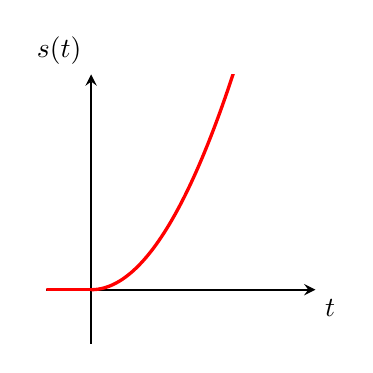
\begin{tikzpicture}
    \begin{axis}
    [	ticks=none,
        axis line style = thick,
        height=5cm,
        width=5cm,
        axis x line=center,
        axis y line=center,
        xmin=-2,
        xmax=10,
        ymin=-0.5,
        ymax=2.0,
        xlabel={$t$},
        ylabel={$s(t)$},
        xlabel style={below right},
        ylabel style={above left},
    ]
    \addplot[instable,domain=-2:0]  {0};
    \addplot[instable,domain=0:10] {0.05*x^2};
    \end{axis}
\end{tikzpicture}

\tikzsetnextfilename{entree_harm-chap0_ext}
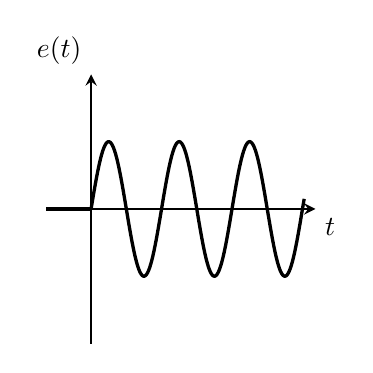
\begin{tikzpicture}
    \begin{axis}
    [   ticks=none,
        axis line style = thick,
        height=5cm,
        width=5cm,
        axis x line=center,
        axis y line=center,
        xmin=-2,
        xmax=10,
        ymin=-2.0,
        ymax=2.0,
        xlabel={$t$},
        ylabel={$e(t)$},
        xlabel style={below right},
        ylabel style={above left},
    ]
    \addplot[entree,domain=-2:0]  {0};
    \addplot[entree,domain=0:9.5]  {sin(deg(2*x))};
    \end{axis}
\end{tikzpicture}
\tikzsetnextfilename{stable_harm-chap0_ext}
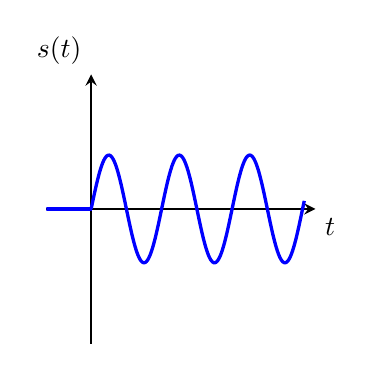
\begin{tikzpicture}
    \begin{axis}
    [   ticks=none,
        axis line style = thick,
        height=5cm,
        width=5cm,
        axis x line=center,
        axis y line=center,
        xmin=-2,
        xmax=10,
        ymin=-2.0,
        ymax=2.0,
        xlabel={$t$},
        ylabel={$s(t)$},
        xlabel style={below right},
        ylabel style={above left},
    ]
    \addplot[stable,domain=-2:0] {0};
    \addplot[stable,domain=0:9.5] {0.8*sin(deg(2*x))};
    \end{axis}
\end{tikzpicture}
\tikzsetnextfilename{instable_harm-chap0_ext}
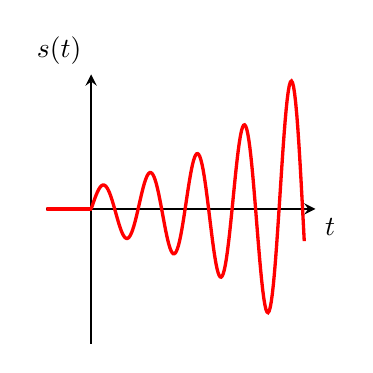
\begin{tikzpicture}%
	\begin{axis}
	[	ticks=none,
        axis line style = thick,
        height=5cm,
        width=5cm,
        axis x line=center,
        axis y line=center,
        xmin=-2,
        xmax=10,
        ymin=-5,
        ymax=5,
        xlabel={$t$},
        ylabel={$s(t)$},
        xlabel style={below right},
        ylabel style={above left},
	]
	\addplot[instable,domain=-2:0] {0};
	\addplot[instable,domain=0:9.5] {0.8*sin(3*deg(x))*exp(0.2*x)};
	\end{axis}
\end{tikzpicture}
